\Minisec{Chord}
Fingertabelle für einen Host A:\\
\begin{tabular}{c|c|c|c}
k & start & end & Node \\
\hline
1	& 	$A_{end}+1$ & nächster Start-1 & Host mit start in Hashtable	\\
2 	&  \dito +1 		&  "				& suche start in Hashtable 	\\
3 	&  \dito +2 		& "					& \\
4  &  \dito +4 			&   "				& \\
k  &  $\cdots$		&  $A_{end}-1$	 	& \\
\end{tabular} \\

\begin{minipage}{0.2\textwidth}
z.B. Fingertabelle für A mit DHT
(Hashlänge = 5 => rechnen mod 32) 

\begin{tabular}{|c|c|c|}
\hline
Knoten & Start & Ende \\
\hline
B & 5 & 14\\
\hline
A & 15 & 20 \\
\hline
C & 21 & 4 \\
\hline
\end{tabular}
\end{minipage} \textbf{$\implies$}
\begin{minipage}{0.25\textwidth}
\begin{tabular}{c|c|c|c}
k & start & end & Node\\
\hline
1	& 	21 & 21 & C\\
2 	&   22 		&  23	&		C		\\
3 	&   24		& 27	&	C \\
4  &  	28		&   3	& C	\\
5 & 4			&	19 &  B
\end{tabular}
\end{minipage}\\

\textbf{Join:} Vorraussetzung: Bekannter Rechner n';

\begin{minipage}{0.5\textwidth}
\begin{enumerate}
\item zuständigkeitsbereich ausrechnen (Hashen der Adresse) und zuständigen Host suchen
\item Fingertabelle anlegen (lookup durch n')
\item Anpassen aller Fingertabellen, die auf den neuen Rechner zeigen \\
(ist abhängig von der größe des übernommenen Hashbereichs)
\item Übernehmen der relevanten Einträge vom bisher zuständigen Host
\end{enumerate}
\end{minipage}\\

\Minisec{CAN}
Abbilden der Hashes auf d Dimensionen\\
Knoten verwaltet Hashes in einem d-Dimensionalen Quader und seine direkten Nachbarn.\\
\textbf{Suche:} Anfrage an den dem Ziel nähesten Nachbarn (Distanz vom Mittelpunkt)\\
\textbf{Join:} wähle zufälligen Punkt, halbiere Bereich (wenn möglich zu Quadraten)	\\
\textbf{Leave:} Übergabe des Quaders an einen Nachbarn \\
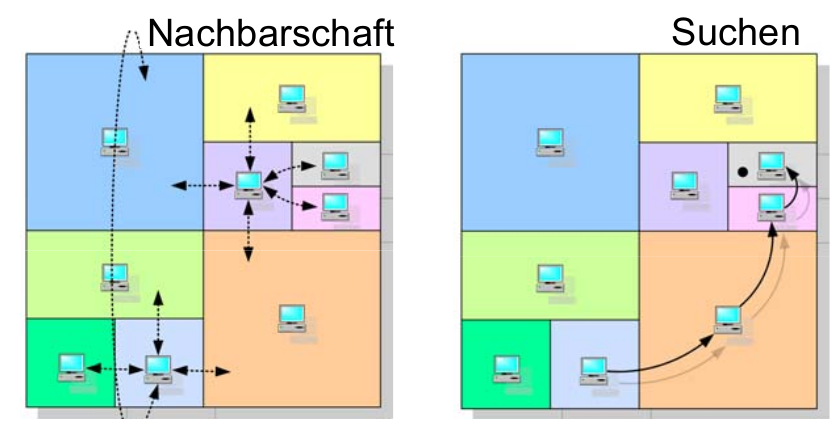
\includegraphics[width=0.35\textwidth]{CAN}

